
%% bare_conf.tex
%% V1.3
%% 2007/01/11
%% by Michael Shell
%% See:
%% http://www.michaelshell.org/
%% for current contact information.
%%
%% This is a skeleton file demonstrating the use of IEEEtran.cls
%% (requires IEEEtran.cls version 1.7 or later) with an IEEE conference paper.
%%
%% Support sites:
%% http://www.michaelshell.org/tex/ieeetran/
%% http://www.ctan.org/tex-archive/macros/latex/contrib/IEEEtran/
%% and
%% http://www.ieee.org/

%%*************************************************************************
%% Legal Notice:
%% This code is offered as-is without any warranty either expressed or
%% implied; without even the implied warranty of MERCHANTABILITY or
%% FITNESS FOR A PARTICULAR PURPOSE! 
%% User assumes all risk.
%% In no event shall IEEE or any contributor to this code be liable for
%% any damages or losses, including, but not limited to, incidental,
%% consequential, or any other damages, resulting from the use or misuse
%% of any information contained here.
%%
%% All comments are the opinions of their respective authors and are not
%% necessarily endorsed by the IEEE.
%%
%% This work is distributed under the LaTeX Project Public License (LPPL)
%% ( http://www.latex-project.org/ ) version 1.3, and may be freely used,
%% distributed and modified. A copy of the LPPL, version 1.3, is included
%% in the base LaTeX documentation of all distributions of LaTeX released
%% 2003/12/01 or later.
%% Retain all contribution notices and credits.
%% ** Modified files should be clearly indicated as such, including  **
%% ** renaming them and changing author support contact information. **
%%
%% File list of work: IEEEtran.cls, IEEEtran_HOWTO.pdf, bare_adv.tex,
%%                    bare_conf.tex, bare_jrnl.tex, bare_jrnl_compsoc.tex
%%*************************************************************************

% *** Authors should verify (and, if needed, correct) their LaTeX system  ***
% *** with the testflow diagnostic prior to trusting their LaTeX platform ***
% *** with production work. IEEE's font choices can trigger bugs that do  ***
% *** not appear when using other class files.                            ***
% The testflow support page is at:
% http://www.michaelshell.org/tex/testflow/



% Note that the a4paper option is mainly intended so that authors in
% countries using A4 can easily print to A4 and see how their papers will
% look in print - the typesetting of the document will not typically be
% affected with changes in paper size (but the bottom and side margins will).
% Use the testflow package mentioned above to verify correct handling of
% both paper sizes by the user's LaTeX system.
%
% Also note that the "draftcls" or "draftclsnofoot", not "draft", option
% should be used if it is desired that the figures are to be displayed in
% draft mode.
%
\documentclass[10pt, conference]{IEEEtran}
% Add the compsocconf option for Computer Society conferences.
%
% If IEEEtran.cls has not been installed into the LaTeX system files,
% manually specify the path to it like:
% \documentclass[conference]{../sty/IEEEtran}





% Some very useful LaTeX packages include:
% (uncomment the ones you want to load)


% *** MISC UTILITY PACKAGES ***
%
%\usepackage{ifpdf}
% Heiko Oberdiek's ifpdf.sty is very useful if you need conditional
% compilation based on whether the output is pdf or dvi.
% usage:
% \ifpdf
%   % pdf code
% \else
%   % dvi code
% \fi
% The latest version of ifpdf.sty can be obtained from:
% http://www.ctan.org/tex-archive/macros/latex/contrib/oberdiek/
% Also, note that IEEEtran.cls V1.7 and later provides a builtin
% \ifCLASSINFOpdf conditional that works the same way.
% When switching from latex to pdflatex and vice-versa, the compiler may
% have to be run twice to clear warning/error messages.






% *** CITATION PACKAGES ***
%
%\usepackage{cite}
% cite.sty was written by Donald Arseneau
% V1.6 and later of IEEEtran pre-defines the format of the cite.sty package
% \cite{} output to follow that of IEEE. Loading the cite package will
% result in citation numbers being automatically sorted and properly
% "compressed/ranged". e.g., [1], [9], [2], [7], [5], [6] without using
% cite.sty will become [1], [2], [5]--[7], [9] using cite.sty. cite.sty's
% \cite will automatically add leading space, if needed. Use cite.sty's
% noadjust option (cite.sty V3.8 and later) if you want to turn this off.
% cite.sty is already installed on most LaTeX systems. Be sure and use
% version 4.0 (2003-05-27) and later if using hyperref.sty. cite.sty does
% not currently provide for hyperlinked citations.
% The latest version can be obtained at:
% http://www.ctan.org/tex-archive/macros/latex/contrib/cite/
% The documentation is contained in the cite.sty file itself.






% *** GRAPHICS RELATED PACKAGES ***
%
\ifCLASSINFOpdf
  % \usepackage[pdftex]{graphicx}
  % declare the path(s) where your graphic files are
  % \graphicspath{{../pdf/}{../jpeg/}}
  % and their extensions so you won't have to specify these with
  % every instance of \includegraphics
  % \DeclareGraphicsExtensions{.pdf,.jpeg,.png}
\else
  % or other class option (dvipsone, dvipdf, if not using dvips). graphicx
  % will default to the driver specified in the system graphics.cfg if no
  % driver is specified.
  % \usepackage[dvips]{graphicx}
  % declare the path(s) where your graphic files are
  % \graphicspath{{../eps/}}
  % and their extensions so you won't have to specify these with
  % every instance of \includegraphics
  % \DeclareGraphicsExtensions{.eps}
\fi
% graphicx was written by David Carlisle and Sebastian Rahtz. It is
% required if you want graphics, photos, etc. graphicx.sty is already
% installed on most LaTeX systems. The latest version and documentation can
% be obtained at: 
% http://www.ctan.org/tex-archive/macros/latex/required/graphics/
% Another good source of documentation is "Using Imported Graphics in
% LaTeX2e" by Keith Reckdahl which can be found as epslatex.ps or
% epslatex.pdf at: http://www.ctan.org/tex-archive/info/
%
% latex, and pdflatex in dvi mode, support graphics in encapsulated
% postscript (.eps) format. pdflatex in pdf mode supports graphics
% in .pdf, .jpeg, .png and .mps (metapost) formats. Users should ensure
% that all non-photo figures use a vector format (.eps, .pdf, .mps) and
% not a bitmapped formats (.jpeg, .png). IEEE frowns on bitmapped formats
% which can result in "jaggedy"/blurry rendering of lines and letters as
% well as large increases in file sizes.
%
% You can find documentation about the pdfTeX application at:
% http://www.tug.org/applications/pdftex





% *** MATH PACKAGES ***
%
%\usepackage[cmex10]{amsmath}
% A popular package from the American Mathematical Society that provides
% many useful and powerful commands for dealing with mathematics. If using
% it, be sure to load this package with the cmex10 option to ensure that
% only type 1 fonts will utilized at all point sizes. Without this option,
% it is possible that some math symbols, particularly those within
% footnotes, will be rendered in bitmap form which will result in a
% document that can not be IEEE Xplore compliant!
%
% Also, note that the amsmath package sets \interdisplaylinepenalty to 10000
% thus preventing page breaks from occurring within multiline equations. Use:
%\interdisplaylinepenalty=2500
% after loading amsmath to restore such page breaks as IEEEtran.cls normally
% does. amsmath.sty is already installed on most LaTeX systems. The latest
% version and documentation can be obtained at:
% http://www.ctan.org/tex-archive/macros/latex/required/amslatex/math/





% *** SPECIALIZED LIST PACKAGES ***
%
%\usepackage{algorithmic}
% algorithmic.sty was written by Peter Williams and Rogerio Brito.
% This package provides an algorithmic environment fo describing algorithms.
% You can use the algorithmic environment in-text or within a figure
% environment to provide for a floating algorithm. Do NOT use the algorithm
% floating environment provided by algorithm.sty (by the same authors) or
% algorithm2e.sty (by Christophe Fiorio) as IEEE does not use dedicated
% algorithm float types and packages that provide these will not provide
% correct IEEE style captions. The latest version and documentation of
% algorithmic.sty can be obtained at:
% http://www.ctan.org/tex-archive/macros/latex/contrib/algorithms/
% There is also a support site at:
% http://algorithms.berlios.de/index.html
% Also of interest may be the (relatively newer and more customizable)
% algorithmicx.sty package by Szasz Janos:
% http://www.ctan.org/tex-archive/macros/latex/contrib/algorithmicx/
\usepackage{amsmath}
\usepackage{centernot}
\usepackage{tikz}
\usepackage{xspace}

% *** ALIGNMENT PACKAGES ***
%
%\usepackage{array}
% Frank Mittelbach's and David Carlisle's array.sty patches and improves
% the standard LaTeX2e array and tabular environments to provide better
% appearance and additional user controls. As the default LaTeX2e table
% generation code is lacking to the point of almost being broken with
% respect to the quality of the end results, all users are strongly
% advised to use an enhanced (at the very least that provided by array.sty)
% set of table tools. array.sty is already installed on most systems. The
% latest version and documentation can be obtained at:
% http://www.ctan.org/tex-archive/macros/latex/required/tools/


%\usepackage{mdwmath}
%\usepackage{mdwtab}
% Also highly recommended is Mark Wooding's extremely powerful MDW tools,
% especially mdwmath.sty and mdwtab.sty which are used to format equations
% and tables, respectively. The MDWtools set is already installed on most
% LaTeX systems. The lastest version and documentation is available at:
% http://www.ctan.org/tex-archive/macros/latex/contrib/mdwtools/


% IEEEtran contains the IEEEeqnarray family of commands that can be used to
% generate multiline equations as well as matrices, tables, etc., of high
% quality.


%\usepackage{eqparbox}
% Also of notable interest is Scott Pakin's eqparbox package for creating
% (automatically sized) equal width boxes - aka "natural width parboxes".
% Available at:
% http://www.ctan.org/tex-archive/macros/latex/contrib/eqparbox/





% *** SUBFIGURE PACKAGES ***
%\usepackage[tight,footnotesize]{subfigure}
% subfigure.sty was written by Steven Douglas Cochran. This package makes it
% easy to put subfigures in your figures. e.g., "Figure 1a and 1b". For IEEE
% work, it is a good idea to load it with the tight package option to reduce
% the amount of white space around the subfigures. subfigure.sty is already
% installed on most LaTeX systems. The latest version and documentation can
% be obtained at:
% http://www.ctan.org/tex-archive/obsolete/macros/latex/contrib/subfigure/
% subfigure.sty has been superceeded by subfig.sty.



%\usepackage[caption=false]{caption}
%\usepackage[font=footnotesize]{subfig}
% subfig.sty, also written by Steven Douglas Cochran, is the modern
% replacement for subfigure.sty. However, subfig.sty requires and
% automatically loads Axel Sommerfeldt's caption.sty which will override
% IEEEtran.cls handling of captions and this will result in nonIEEE style
% figure/table captions. To prevent this problem, be sure and preload
% caption.sty with its "caption=false" package option. This is will preserve
% IEEEtran.cls handing of captions. Version 1.3 (2005/06/28) and later 
% (recommended due to many improvements over 1.2) of subfig.sty supports
% the caption=false option directly:
%\usepackage[caption=false,font=footnotesize]{subfig}
%
% The latest version and documentation can be obtained at:
% http://www.ctan.org/tex-archive/macros/latex/contrib/subfig/
% The latest version and documentation of caption.sty can be obtained at:
% http://www.ctan.org/tex-archive/macros/latex/contrib/caption/




% *** FLOAT PACKAGES ***
%
%\usepackage{fixltx2e}
% fixltx2e, the successor to the earlier fix2col.sty, was written by
% Frank Mittelbach and David Carlisle. This package corrects a few problems
% in the LaTeX2e kernel, the most notable of which is that in current
% LaTeX2e releases, the ordering of single and double column floats is not
% guaranteed to be preserved. Thus, an unpatched LaTeX2e can allow a
% single column figure to be placed prior to an earlier double column
% figure. The latest version and documentation can be found at:
% http://www.ctan.org/tex-archive/macros/latex/base/



%\usepackage{stfloats}
% stfloats.sty was written by Sigitas Tolusis. This package gives LaTeX2e
% the ability to do double column floats at the bottom of the page as well
% as the top. (e.g., "\begin{figure*}[!b]" is not normally possible in
% LaTeX2e). It also provides a command:
%\fnbelowfloat
% to enable the placement of footnotes below bottom floats (the standard
% LaTeX2e kernel puts them above bottom floats). This is an invasive package
% which rewrites many portions of the LaTeX2e float routines. It may not work
% with other packages that modify the LaTeX2e float routines. The latest
% version and documentation can be obtained at:
% http://www.ctan.org/tex-archive/macros/latex/contrib/sttools/
% Documentation is contained in the stfloats.sty comments as well as in the
% presfull.pdf file. Do not use the stfloats baselinefloat ability as IEEE
% does not allow \baselineskip to stretch. Authors submitting work to the
% IEEE should note that IEEE rarely uses double column equations and
% that authors should try to avoid such use. Do not be tempted to use the
% cuted.sty or midfloat.sty packages (also by Sigitas Tolusis) as IEEE does
% not format its papers in such ways.

\newif\ifdraft
\drafttrue

\input{macros}



% *** PDF, URL AND HYPERLINK PACKAGES ***
%
\usepackage{url}
% url.sty was written by Donald Arseneau. It provides better support for
% handling and breaking URLs. url.sty is already installed on most LaTeX
% systems. The latest version can be obtained at:
% http://www.ctan.org/tex-archive/macros/latex/contrib/misc/
% Read the url.sty source comments for usage information. Basically,
% \url{my_url_here}.





% *** Do not adjust lengths that control margins, column widths, etc. ***
% *** Do not use packages that alter fonts (such as pslatex).         ***
% There should be no need to do such things with IEEEtran.cls V1.6 and later.
% (Unless specifically asked to do so by the journal or conference you plan
% to submit to, of course. )


% correct bad hyphenation here
\hyphenation{op-tical net-works semi-conduc-tor}


\begin{document}
%
% paper title
% can use linebreaks \\ within to get better formatting as desired
\title{How much time did it take to notify a Bug? \\ Two case studies: ElasticSearch and Nova}


% author names and affiliations
% use a multiple column layout for up to two different
% affiliations

\author{\IEEEauthorblockN{Gema Rodriguez-Perez}
\IEEEauthorblockA{GSyC/LibreSoft\\
Universidad Rey Juan Carlos\\
Fuenlabrada, Spain\\
gerope@libresoft.info}
\and
\IEEEauthorblockN{Gregorio Robles}
\IEEEauthorblockA{GSyC/LibreSoft\\
Universidad Rey Juan Carlos\\
Fuenlabrada, Spain\\
grex@gsyc.urjc.es}
\and
\IEEEauthorblockN{Jesus M. Gonzalez-Barahona}
\IEEEauthorblockA{GSyC/LibreSoft\\
Universidad Rey Juan Carlos\\
Fuenlabrada, Spain\\
jgb@gsyc.es}
}

% conference papers do not typically use \thanks and this command
% is locked out in conference mode. If really needed, such as for
% the acknowledgment of grants, issue a \IEEEoverridecommandlockouts
% after \documentclass

% for over three affiliations, or if they all won't fit within the width
% of the page, use this alternative format:
% 
%\author{\IEEEauthorblockN{Michael Shell\IEEEauthorrefmark{1},
%Homer Simpson\IEEEauthorrefmark{2},
%James Kirk\IEEEauthorrefmark{3}, 
%Montgomery Scott\IEEEauthorrefmark{3} and
%Eldon Tyrell\IEEEauthorrefmark{4}}
%\IEEEauthorblockA{\IEEEauthorrefmark{1}School of Electrical and Computer Engineering\\
    %Georgia Institute of Technology,
%Atlanta, Georgia 30332--0250\\ Email: see http://www.michaelshell.org/contact.html}
%\IEEEauthorblockA{\IEEEauthorrefmark{2}Twentieth Century Fox, Springfield, USA\\
%Email: homer@thesimpsons.com}
%\IEEEauthorblockA{\IEEEauthorrefmark{3}Starfleet Academy, San Francisco, California 96678-2391\\
%Telephone: (800) 555--1212, Fax: (888) 555--1212}
%\IEEEauthorblockA{\IEEEauthorrefmark{4}Tyrell Inc., 123 Replicant Street, Los Angeles, California 90210--4321}}




% use for special paper notices
%\IEEEspecialpapernotice{(Invited Paper)}




% make the title area
\maketitle


\begin{abstract}

The \emph{Time To Notify} (TTN) a bug is a valuable metric in the software maintenance and evolution studies that describes how much time it takes for a bug to be notified/reported in the issue tracking system since the time the bug was introduced into the source code. Even so, it is still a challenge to exactly calculate it since no precise way exists to locate where and when the bug originated. This paper aims to study what is the value of TTN in two different projects. For a set of bugs in these projects, we know exactly which ``previous commit'' was the cause of the failure in the system. Furthermore, to better understand how this is related to the maintenance and evolution of a software, we also analyze the relationship between TTN and other metrics extracted from the source code management (SCM) system such as the author of the bug, the \emph{Time To Fix} (TTF) or the developer experience.
We have observed that the mean of the TTN in the projects was 312 days and 431 days. However, only one of the projects showed a moderate correlation between the experience of the author who created the bug and TTN.
\end{abstract}

\begin{IEEEkeywords}
Bug introduction change; bug seeding metrics;

\end{IEEEkeywords}


% For peer review papers, you can put extra information on the cover
% page as needed:
% \ifCLASSOPTIONpeerreview
% \begin{center} \bfseries EDICS Category: 3-BBND \end{center}
% \fi
%
% For peerreview papers, this IEEEtran command inserts a page break and
% creates the second title. It will be ignored for other modes.
\IEEEpeerreviewmaketitle



\section{Introduction}
\label{sec:intro}

It is well-known that a large amount of the total effort of a software system is spent in maintenance and evolution~\cite{tassey2002economic}, some sources even assigning this phase over 80\% of the total cost. Hence, researchers have spent much effort understanding and characterizing software maintenance and evolution processes. One of the main areas in software maintenance and evolution is related to bug detection and analysis. Metrics such as the \emph{Time To Fix} (TTF), the \emph{Time To Review} (TTR) or the \emph{fix-effort} to improve code quality have been thus proposed in the research literature~\cite{kim2006long}\cite{mockus2002two}. One of these metrics, the one that this paper is going to analyze is the the \emph{Time To Notify} (TTN) a bug. The TTN is the time that goes from the time where a bug has been introduced in the source code to the time when the wrong behavior is notified in the bug tracking system of a project. 
\gema{Review 1 said that we should improve the motivation}

The concept of TTN provides insight into fundamental aspects of the software maintenance of a project that are not easy to obtain, especially in Free/Open Source Software (FOSS) communities -- such as the well-known Mozilla, Eclipse or GNOME projects. In these environments, effort information has historically neither been stored nor maintained in their bug tracking system (e.g., Bugzilla) in spite of the valuable knowledge of the product complexity that it  could provide. Currently, the only bug tracking system that allows store and maintain some type of effort information related to bug fixing activity is JIRA~\cite{weiss2007long}, as it includes an estimate of the time it will take to fix the issue. However, the TTN can be potentially calculated by combining information from the source code management system (SCM) and bug tracking system (BTS). Although it won't directly provide a measure of (human) effort, it is a proxy of efficiency: low values of TTN means a better maintained software (with code being changed/tested continuously), while higher values may denote less maintained software (with potential risks being present for longer periods of time).
\gema{Review 1 said that the paper needs writing some examples or scenarios where TTN could be useful}

To compute the life of a bug in a software, it is necessary to know exactly when and where a bug was introduced. As versioning systems (such as git) are commonly used in modern software development, meta-data (committer, author, time, etc.) on all changes exists, and we could potentially identify what line introduced the bug. However, finding the line of code where the bug was introduced is not a trivial task. Several methods have been proposed to determine what commits are the candidates of having introduced a given bug. The popular SZZ algorithm~\cite{sliwerski2005changes} is one of them: it traces the lines touched in a \emph{fixing} commit back to the time when these lines were modified or added. The main concern in using this algorithm is the that it is prone to provide a wrong measure in some situations that frequently happen during the evolution of a software system. These situations, such as changes in the API, present a common characteristic: the bug was not introduced in the previous commit(s). So, when the line was introduced, the software was correct; the wrong behavior appears due to other, external changes.


In this paper, we measure TTN for a set of bugs from two different FOSS projects: ElasticSearch and Nova. Because of previous research performed on them by the authors, we know the exact location of the \emph{Bug Introducing Change} (BIC) for a set of bugs. This means that from a set of ``previous commits'' of each of the fixing lines, we are able to identify what specific previous commit caused the failure in the system.

Furthermore, to better understand how this is related to the maintenance and evolution of a software, we also analyze the relationship between TTN and other metrics extracted from the SCM system, such as the author of the bug, the time to fix or the developer experience inserting the bug.

Summing up, we are interested in studying the \emph{real} value of TTN to answer following research questions:
\begin{itemize}
  \item RQ1: What are the values of TTN in both projects? What is its mean, median, etc.?
  \item RQ2: What is the correlation of TTN with others characteristics of the project/developers involved in the bug fixing process? 
\end{itemize}
\gema{Review 1 said that we should clarify how important are RQ1 and RQ2 for researchers and practitioners}

Our results reveal that the mean TTN differs from the mean calculated with other methods. In addition, we have found that TTN has a dependency with the experience of the developer who introduced the bug. On the other hand, we note that to measure the TTN is crucial to determine exactly the location of the BIC; so far, now no precise way exists. Thus, we propose a simple idea which may shed some light to this problem.

%Our main findings reveal that the \emph{real} mean TTN ranges from ten months in ElasticSearch to fourteen months in Nova. If we compare our results with the ones obtained with applying the SZZ algorithm, in the optimistic approach (i.e., considering the newest ones) the mean TTN in Nova is eight months and in ElasticSearch five months and in the pessimistic one (i.e., considering the oldest ones) the mean in Nova is thirteen months and twelve months in ElasticSearch. On the other hand, only one of the projects showed a weak correlation between TTN and the experience of the author who introduced the bug. \grex{If it is not completely clear, then we should skip this paragraph. For instance, the reader does not know what optimistic and pessimistic SZZ is at this time. We should focus really more on the contributions than on the results, which are given later!}

The remainder of the paper is organized as follows: In Section~\ref{sec:relatedwork} the current body of knowledge is presented. Next, Section~\ref{sec:methodology} describes the methodology used to identify the Bug Introducing Change (BIC) and calculates the metrics. Results obtained for Nova and ElasticSearch are presented in Section~\ref{sec:results}. Section~\ref{sec:discussion} answers the research questions, and discusses potential applications and improvements to our approach. After reporting the limitations and threats to validity in Section~\ref{sec:threats}, we draw some conclusions and point out potential future work in Section~\ref{sec:conclusions}.

\section{Related Work}
\label{sec:relatedwork}


Kim and Whitehead calculated the time to fix bugs (\emph{bug-fix time}) in ArgoUML and PostgreSQL projects reporting that the median time for fixing a single bug is around 200 days. Also, they argue that this time is a significant factor to measure the quality of a software system~\cite{kim2006long}. Furthermore, Guo \emph{et al.} studied two Microsoft products, looking for the attributes that had influence in the fixing commit: they found that bugs reported by developers with higher reputation were not only more likely to get fixed, but also fixed faster~\cite{guo2010characterizing}.

Eyolfson \emph{et al.} define the (\emph{bug-fix time}) as the time from the earliest commit that introduced the bug to the bug-fixing commit. Their findings show that the time and day of a code commit may affect the quality of the code~\cite{eyolfson2011time}.

Lionel \emph{et al.} also studied the fix-time for Bugs in large FOSS projects; their results indicate that the priority of a bug in Eclipse is correlated with the time to fix~\cite{marks2011studying}. On the contrary, Bhattacharya \emph{et al.} used regression testing to measure the correlation between bug-fix time with some of the bug report attributes such as number of attachments or bug severity, finding that their results did not present such correlation~\cite{bhattacharya2011bug}.

%Lehtonen \emph{et al.} studied the review process in Gerrit and introduced some metrics such as the review time, integration time or average number of patch-sets explaining that monitoring the code review process is not as easy as was we could think~\cite{lehtonen2015metrics}.

%Authors ~\cite{zhang2012empirical} studied which factors affect in the delayed time incurred by developers from the bug was opened until the fixing activity started. Their explanation to this delay was the: Type, Severity, Operating System, Property of Code or Comments of a Bug~\cite{zhang2012empirical} 

Zhang \emph{et al.} proposed an effective method for predicting the number of bugs that will be fixed in the future and the time required and \emph{quickness}, a binary classification (slow or quick) of the time required to fix a bug~\cite{zhang2013predicting}. In this line Ginger \emph{et al.} investigated the relationship between bug report attributes in three FOSS projects --Eclipse, Mozilla, and GNOME-- to build a prediction model. Their findings show that the reporter, the assignee and the date the bug report was opened were the attributes with the strongest influence on the fix-time of the bugs~\cite{giger2010predicting}.


Some authors have decided to study how the experience of the author affects in the bug fixing activity. Development experience has been measured in several ways: number of commits~\cite{eyolfson2011time}, fixing activity~\cite{ahsan2010mining} and ownership~\cite{german2004using}. Thus, based on these measures, Izquierdo \emph{et al.} analyzed some Mozilla modules expecting statistical differences between developers with different levels of experience and the introduction of bugs, but the results did not show correlation, meaning that more experience does not imply less bug introducing changes~\cite{izquierdo2012more}. Also, Izquierdo \emph{et al.} studied whether developers who introduced a bug were the same who fixed it; their findings show that in most cases people are usually fixing bugs that were introduced by other developers~\cite{izquierdo2011developers}.

Other studies have analyzed the experience of the author to predict the future bugs, and although there is research literature that suggests that by using this information the prediction of bugs does not improve~\cite{weyuker2010programmer}, others report that the change's defect probability decreases with higher experience of the developers~\cite{mockus2000predicting}. However, it seems there is evidence that defect injection rates vary among different developers~\cite{matsumoto2010analysis}.


While the prior studies were built under the assumption that the previous modifications to a fixed line was the cause of the bug, the contribution of our study resides in the fact that we do not follow this assumption, which is sometimes flawed. Instead, we identify the \emph{real} modification that introduced the bug~\cite{rodriguez2016bugtracking}. Once this modification is identified, we compute some of the metrics found in previous studies and compare our results to them.

\section{Methodology}
\label{sec:methodology}

In our study, the data analyzed has been obtained from the source code management system, the issue tracking system and the code review system. We illustrate our methodology in Figure~\ref{fig:methodology}, where the input is a set of bug reports randomly extracted from the issue tracking system. The steps of our process are given by white boxes; the colored boxes give the sources that have been used to obtain the information required in each step.
\gema{Review 1 said that we need to write how bug reports and fixing commits are linked, maybe with an additional step in figure~\ref{fig:methodology}}
\begin{figure}[ht]
\centering
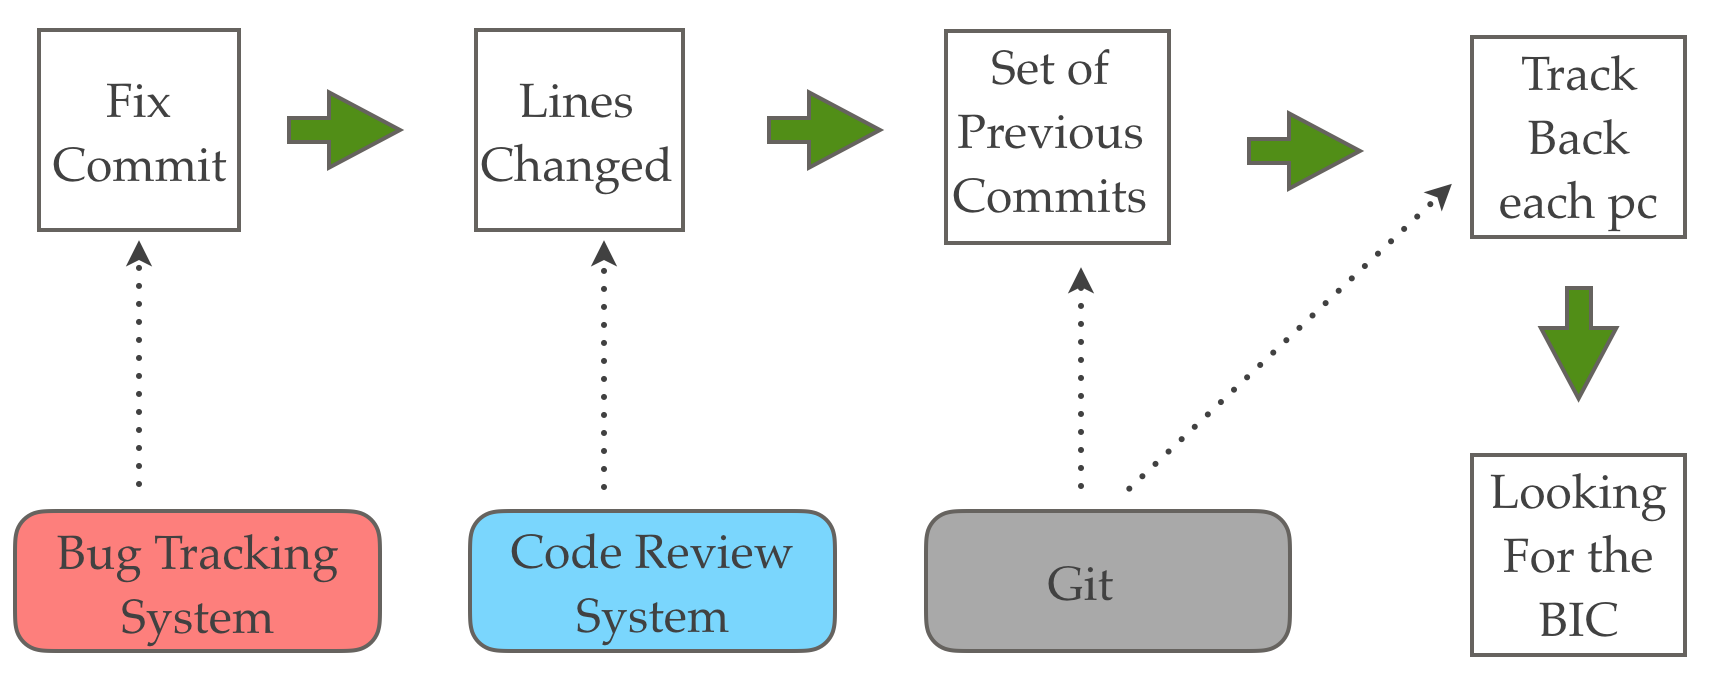
\includegraphics[width=\columnwidth]{methodology.png}
\caption{The methodology used in this study, starting with the analysis of a fixing commit, determining the involved lines of code, obtaining the previous commits, finding the BIC and finally computing the value of the metrics for the whole process.}
\label{fig:methodology}       % Give a unique label
\end{figure}

The following list is a detailed description of the steps: 

\begin{enumerate}
		\item Find the fixing commit of each bug report.
		\item Find the lines that this commit added, modified or deleted to solve the bug.
		\item Obtain, for each of those lines, the commit that added, modified or deleted these lines previously. The result is a set with \emph{previous commits} for each line.
		\item Analyze which one of the previous commits was the BIC. In the case where the preceding commit is not the origin of the bug track back to a previous commit, until the line causing the failure is found. In the case where the fixing commit consist exclusively of new lines, analyze previous commits to nearby lines looking whether in any of them the developer \emph{forgot} to add these lines. It should be noted that the SZZ algorithm discards fixing commits that only add lines.
		\item Extract the date when the fixing commit, the BIC and the bug report have been submitted, as well as the author of each of the commits to calculate our metrics.	
\end{enumerate} 


\subsection{Metrics}

To compute the metrics used in this study, we need to identify the BIC. Once this has been done, we are able to measure the time values. Next, we describe the metrics used in our study: 

\begin{itemize}
		\item \emph{Experience until Bug Introducing Change} (EuBIC): Experience of the author of the BIC at the moment of doing the commit. Experience is measured in days from the first time that the author committed some code to the project until the BIC.
		\item \emph{Time To Notify} (TTN): Time in days since the bug introducing commit was merged into the master branch until some developer notified the unexpected behavior and reported it in the bug tracking system. 
		\item \emph{Time To Fix} (TTF): Period in days from the notification of a bug report to when it was closed with a fixing commit.
		\item \emph{Bug Fixing Time} (BFT): Time in days from the date of the BIC to the fixing commit date. This value can be also computed by adding TTN and TTF.
\end{itemize} 

Figure~\ref{fig:metrics} provides a visual explanation of the metrics proposed in this paper. For example, to obtain the metrics for bug report \#13334 of ElasticSearch, we need to identify the fixing commit (which is $c6da8d5e1$) and the BIC ($c73fff7$). Then, analyzing the meta-data of theses commits, we obtain the date and the author for both of them: the bug report was done in September 4\textsuperscript{th} 2015, the fixing commit in  September 15\textsuperscript{th} 2015, and the BIC was inserted in July 13\textsuperscript{th}  2015 by a developer with almost 3 years of experience in the project. Hence, in our example, the values of the metrics under study are: 54 days for TTN, 11 days for TTF, 65 days for BFT and 1,097 days for EuBIC.
\begin{figure}[ht]
\centering
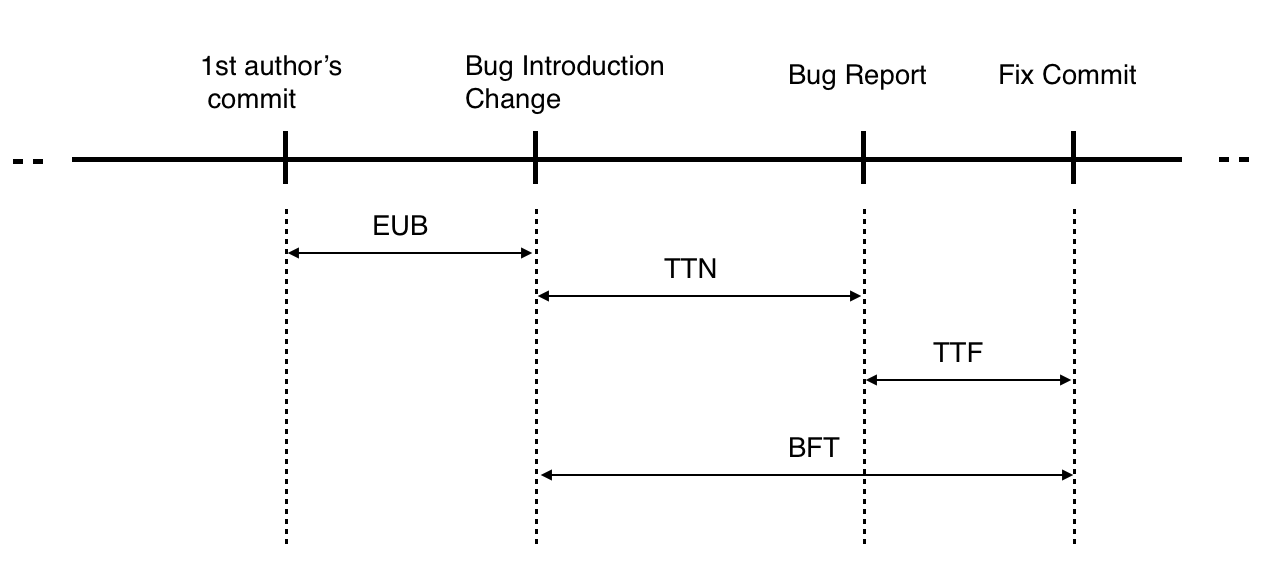
\includegraphics[width=\columnwidth]{metrics.png}
\caption{Visualization of the periods under study: Experience Until Bug Introducing Change (EuBIC),  Time To Notify (TTN), Time To Fix (TTF), Bug Fixing Time (BFT).}
\label{fig:metrics}       % Give a unique label
\end{figure}

\gema{Review 1 said that the comparison with SZZ should be mentioned earlier in the paper (goal/contribution)}
We would like to compare our metrics with the widely used SZZ algorithm. We will therefore assume that the closest commit in time (i.e., the previous one) of the SZZ algorithm is the one that induces the bug-fixing commit, as it has been done in previous works~\cite{eyolfson2011time}. It should be noted, however, that the SZZ algorithm may not identify the BIC correctly, as its outcome could be a set of commits among which the \emph{real} BIC is not included. In addition, in our comparison we discard those fixing commits with only new lines, since the SZZ algorithm removes them from the analysis.


\section{Evaluation}
\label{sec:evaluation}

We have validated our methodology analyzing tickets from two projects, Nova and ElasticSearch, written in different programming languages. %Nova uses Python, an interpreted language, whereas ElasticSearch uses Java, a compiled language.  Thus, we can study the dependency of TTN with the programming language that the project is using.
\gema{Review 1 said that we have missed talk about which correlation tests have been used}
Nova belongs to the OpenStack project, a cloud computing platform with a huge developer community (more than 5,000 developers) and significant industrial support from hundreds of organizations, among them several major IT companies such as Red Hat, Intel, IBM, HP, etc. The source code of Nova is written in Python and was particularly of interest because it is continuously evolving due to its very active community. Currently it has more than 44,000 commits with more than 2 million lines of code and around 1,000 contributors\footnote{\url{http://activity.openstack.org/dash/browser/repository.html?repository=nova.git&ds=scm}}. All its code is hosted and available in GitHub\footnote{\url{https://github.com/openstack/nova}} and it is developed with git\footnote{\url{https://git-scm.com/}} as the source code management, Launchpad\footnote{\url{https://launchpad.net/}} as the issue tracking system and Gerrit\footnote{\url{https://www.gerritcodereview.com/}} as the code review system.

ElasticSearch is a distributed FLOSS search and analytics engine written in Java. It has 26,000 commits and 764 contributors. Its labeling policy in the bug tracking system is very strict, thus we can be sure that tickets labeled as bug reports (i.e., the ones analyzed in this paper) are \emph{real} bug reports. ElasticSearch hosts its code in GitHub\footnote{\url{https://github.com/elastic/elasticsearch/}}. The project uses GitHub's issue tracking and pull request system for bug tracking and reviewing.
\gema{Review 1 said that we should detail the research questions, describing the statistical tests used to answer this questions}
We use in this paper a data set from these two projects created in a prior research work, where we manually analyzed a total of 76 bug fixing commits of real bug reports in detail, looking in each one for the BIC that caused the failure~\cite{gema2016doctoral}. %Thus, once we have the commit that induced the later fix, we calculate the values of the TTN, EuBIC, TTF and the authors of the fixing commit, the bug report, and the bug introducing change.  


\section{Results}
\label{sec:results}

We have calculated the values of TTN, EuBIC and TTF for 76 bug fixing commits, 39 belonging to Nova and 37 belonging to ElasticSearch. %In addition, we compare these values with the values resulting from the SZZ algorithm.
\gema{Review 2 said that a key statistic table for each dataset could be useful}
Table~\ref{tableNova} and Table~\ref{tableES} show the means of Time To Notify (TTN), Time To Fix (TTF) and Bug Fixing Time (BFT) computed for the Nova and the ElasticSearch projects, respectively. The tables include the values for the \emph{real} BIC (manually checked), and the ones that can be obtained by using the SZZ algorithm.

\begin{table}[!t]
% increase table row spacing, adjust to taste
\renewcommand{\arraystretch}{1.3}
\centering
\caption{Mean in days of TTN, TTF, BFT for the Nova project, both for the \emph{real} BIC as for the BIC obtained with SZZ}
\label{tableNova}
% Some packages, such as MDW tools, offer better commands for making tables
%% than the plain LaTeX2e tabular which is used here.
\begin{tabular}{|c||c||c||c| }
\hline
  & TTN & TTF & BFT \\
\hline
Real & 432 & 65 & 497 \\
\hline
SZZ & 260 & 52 & 312\\
\hline
\end{tabular}
\end{table}

\begin{table}[!t]
% increase table row spacing, adjust to taste
\renewcommand{\arraystretch}{1.3}
\centering
\caption{Mean in days of TTN, TTF, BFT for the ElasticSearch project, both for the \emph{real} BIC as for the BIC obtained with SZZ.}
\label{tableES}
% Some packages, such as MDW tools, offer better commands for making tables
%% than the plain LaTeX2e tabular which is used here.
\begin{tabular}{|c||c||c||c| }
\hline
  & TTN & TTF & BFT \\
\hline
Real & 312 & 14 & 326 \\
\hline
SZZ & 135 & 16 & 151\\
\hline
\end{tabular}
\end{table}

Figure~\ref{fig:meansOfNova} and Figure~\ref{fig:meansOfES} show the values of TTN, TTF and EuBIC for both projects using box plots. We can see that it takes 158 days in ElasticSearch to notify 50\% of the bugs, and 336 days for Nova. The mean is almost 200 days in ElasticSearch and around 350 days in Nova. TTF is low for both projects, but especially for ElasticSearch where there is almost no dispersion and bugs are fixed almost immediately after their notification. And Nova developers are slightly more experienced than ElasticSearch developers when they introduce bugs.

\begin{figure}[ht]
\centering
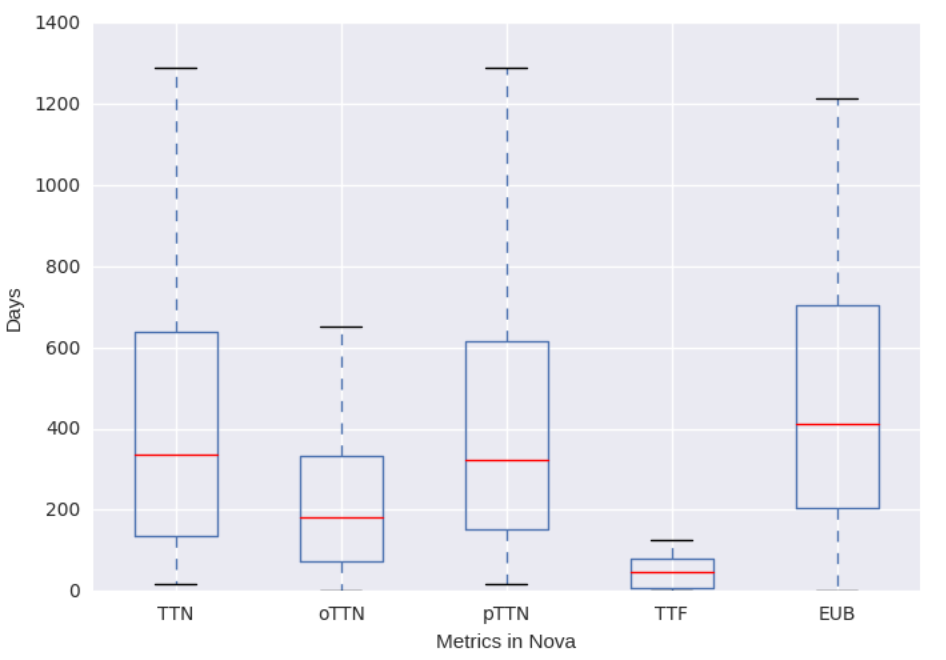
\includegraphics[width=\columnwidth]{boxplotNova.png}
\caption{Box-plots with TTN, TTF and EuBIC for the Nova project.}
\label{fig:meansOfNova}       % Give a unique label
%\caption{Box-Plot in Nova}
%\label{fig:graph4}       % Give a unique label
\end{figure}

\begin{figure}[ht]
\centering
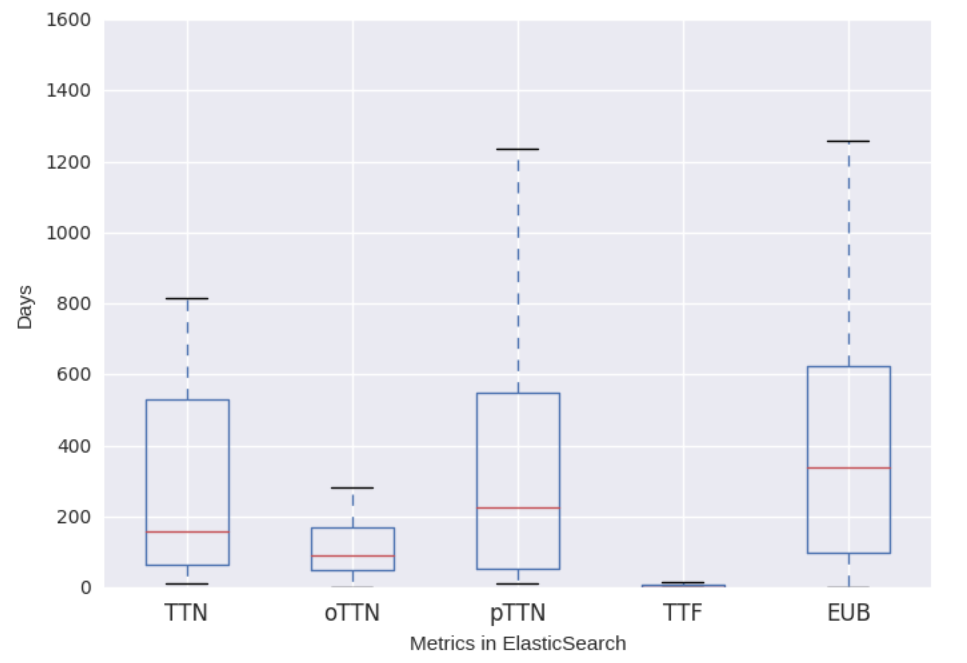
\includegraphics[width=\columnwidth]{boxplotES.png}
\caption{Box-plots with TTN, TTF and EuBIC for the ElasticSearch project.}
\label{fig:meansOfES}       % Give a unique label
%\caption{Box-Plot in ES}
%\label{fig:graph5}       % Give a unique label
\end{figure}

Figure~\ref{fig:correlation} shows the correlation matrix between the metrics under analysis for the Nova project. A moderate negative correlation, $-0.56$, between the EuBIC of the author introducing the bug and TTN can be found. The value of this correlation for the ElasticSearch project is $-0.383$, which points to a weaker relationship\footnote{Due to space constrains we do not show a similar figure for ElasticSearch.}.\gema{Review 2 said that why there is no corresponding diagram (correlation) for the ES}

\begin{figure}[ht]
\centering
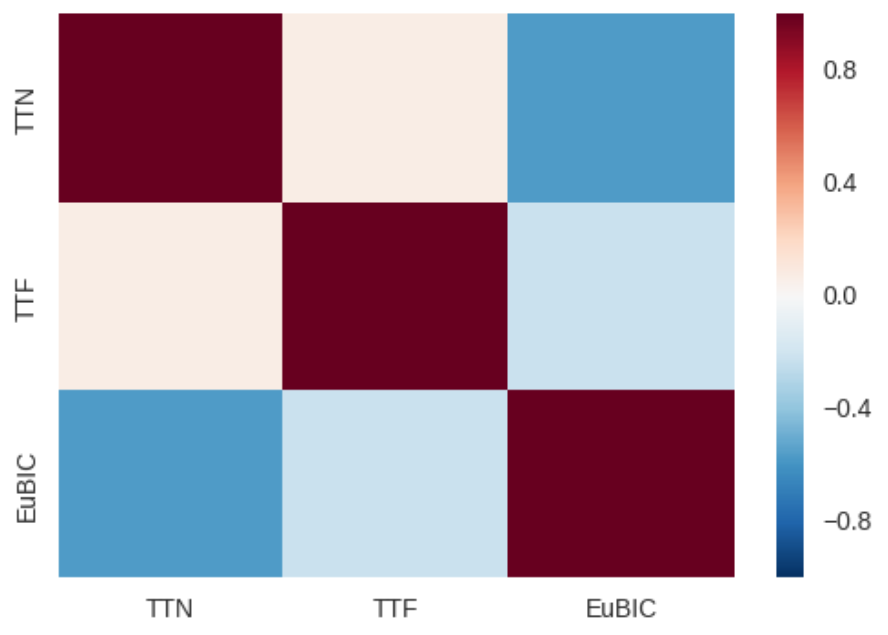
\includegraphics[width=\columnwidth]{correlationMatrix.png}
\caption{Correlation Matrix of the variables measured for the Nova project. Correlation coefficients are colored according to the value; white means a correlation value of 0, the red tone increases with the grade of positive correlation while the blue tone decreases with the grade of negative correlation.}
\label{fig:correlation}       % Give a unique label
\end{figure}

Figure~\ref{fig:graph} shows scatterplots with the distribution of each pair of metrics for the Nova project. While we can infer a negative inclination in the relationship between TTN and EuBIC with a $R^2$ value of 0.32, which indicates how closely these two variables are related, the plot for TTN or EuBIC against TTF does not indicate such tendency. 

\begin{figure}[ht]
\centering
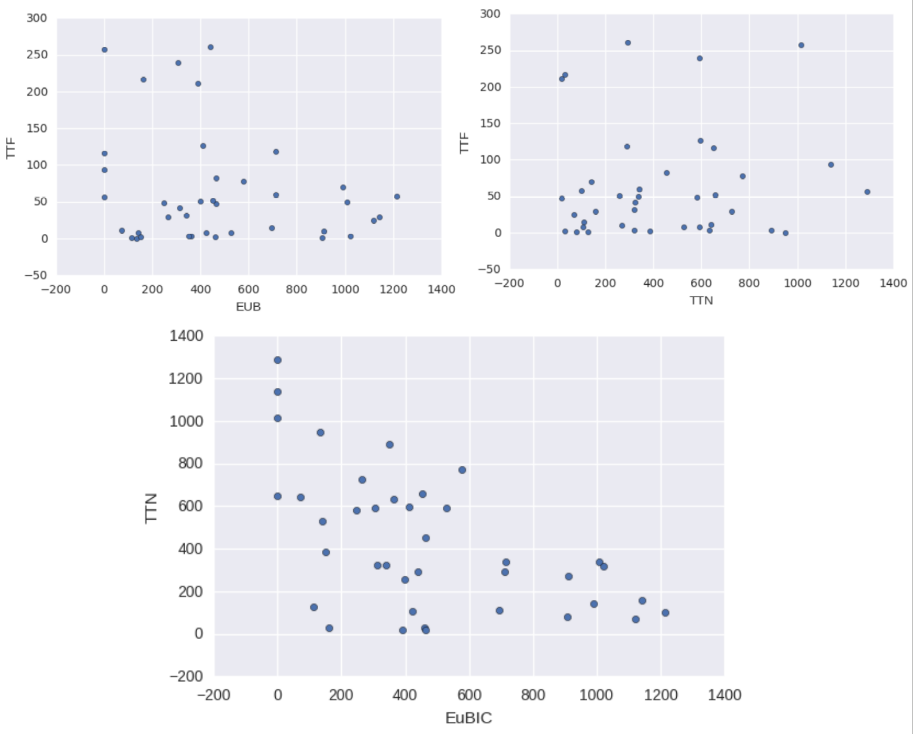
\includegraphics[width=\columnwidth]{DistributionNova_b.png}
\caption{ Scatterplots with the metrics for the Nova project.}
\label{fig:graph}       % Give a unique label
\end{figure}

On the other hand, Figure~\ref{fig:graph1} shows how the variables are related to each other in ElasticSearch. In this project, it is difficult to notice the how closely the variables are related, the value of the coefficient $R^2$ in each scatterplot is around 0.09. 

\begin{figure}[ht]
\centering
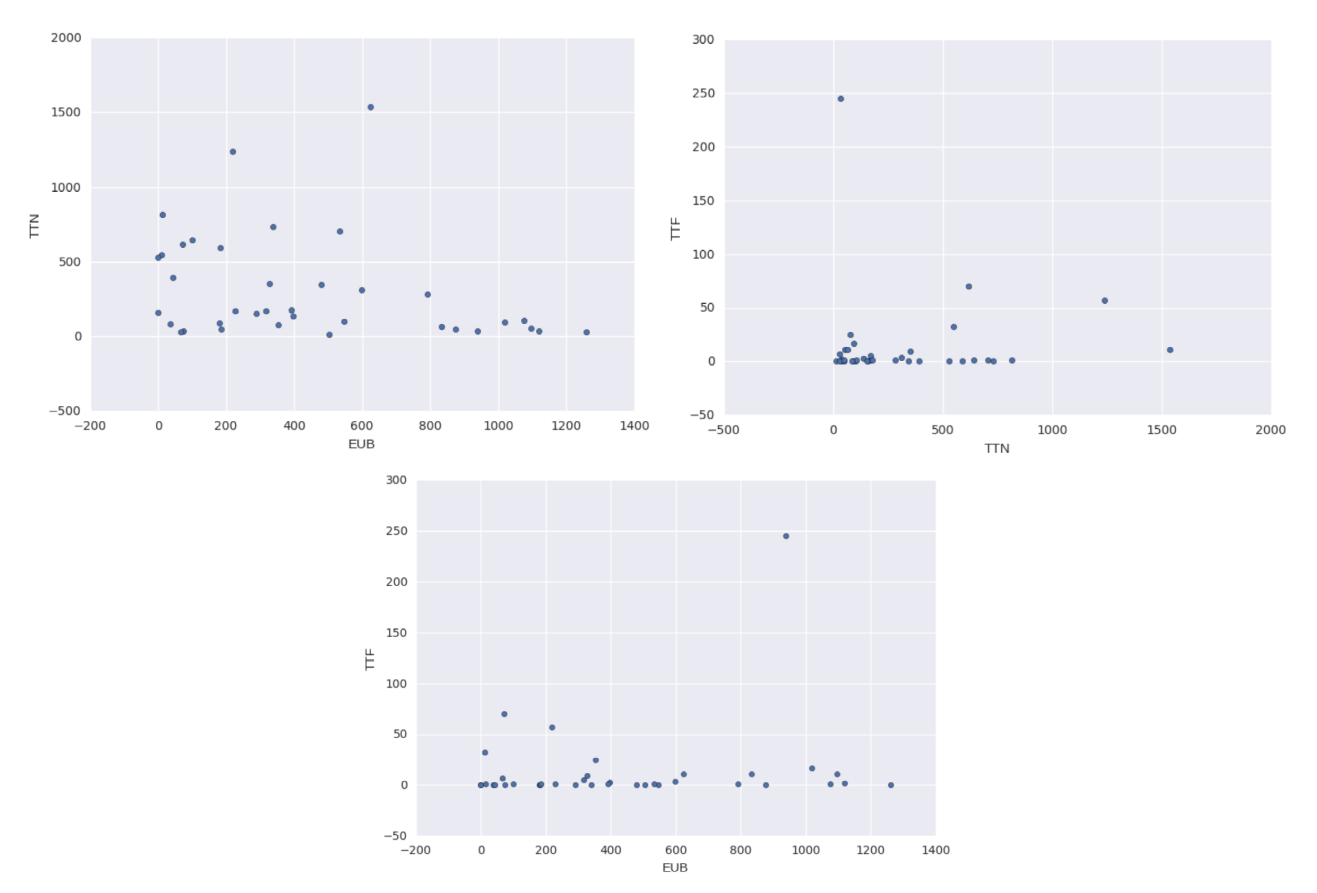
\includegraphics[width=\columnwidth]{DistributionES_b.png}
\caption{Scatterplots with the metrics for the ES project.}
\label{fig:graph1}       % Give a unique label
\end{figure}


To gain further insight into the problem, we have analyzed if the same person who introduced the BIC is also the one who reported and/or fixed it. Tables~\ref{tableII} and~\ref{tableIII} show the percentage of bugs in ElasticSearch and Nova where the same developer (1) notified and fixed the bug, (2) introduced the BIC and fixed the bug, (3) introduced the BIC and notified the bug, and (4) introduced the BIC, notified the bug and fixed it.

The highest percentage corresponds to the situation where the same developer who notifies the bug also fixes it. The second rank is for bugs that have been fixed by the same developer who introduced it, i.e., somebody else reported the bug; in the case of ElasticSearch, the percentage is as high as for the previous case. The cases where the same developer introduced the bug and later on notified it are less frequent, but still happen often (30\% for ElasticSearch and 13\% for Nova). Finally, a bug introduced, notified and fixed by the same developer occurs not marginally (25\% for ElasticSearch, 13\% for Nova).

\begin{table}[!t]
% increase table row spacing, adjust to taste
\renewcommand{\arraystretch}{1.3}
\centering
\caption{Percentage of bugs where a developer performed more than one of the tasks under study (introduce, notify, fix) for the ElasticSearch project.}
\label{tableII}
% Some packages, such as MDW tools, offer better commands for making tables
%% than the plain LaTeX2e tabular which is used here.
\begin{tabular}{|c||c||c||c||c| }
\hline
  & Notify-Fix & Introd.-Fix & Introd.-Notify &  Introd.-Notify-Fix \\
\hline
Yes & 16 (43\%) & 16 (43\%) & 11 (30\%) & 10 (27\%) \\
\hline
No & 21 (57\%) & 21 (57\%) & 26 (70\%) & 27 (73\%) \\
\hline
\end{tabular}
\end{table}

\begin{table}[!t]
% increase table row spacing, adjust to taste
\renewcommand{\arraystretch}{1.3}
\centering
\caption{Percentage of bugs where a developer performed more than one of the tasks under study (introduce, notify, fix) for the ElasticSearch project.}
\label{tableIII}
% Some packages, such as MDW tools, offer better commands for making tables
%% than the plain LaTeX2e tabular which is used here.
\begin{tabular}{|c||c||c||c||c| }
\hline
  & Notify-Fix & Introd.-Fix & Introd.-Notify & Introd.-Notify-Fix \\
\hline
Yes & 30 (77\%) & 7 (18\%) & 5 (13\%) & 5 (13\%) \\
\hline
No & 9 (23\%) & 32 (82\%) & 34 (87\%) &  34 (87\%) \\
\hline
\end{tabular}
\end{table}


\section{Discussion}
\label{sec:discussion}
\gema{Review 1 said that we should discuss the findings in a qualitative way}
After analyzing several fixing commits in this study, we have seen that the \emph{real} (manually validated) TTN differs from the one computed using the well-known and widely-used SZZ algorithm substantially, identifying different BICs in 36\% of the cases in Nova and in 24\% in ElasticSearch. This is the reason why the mean TTN computed using SZZ is almost half the \emph{real} one. %The principal reasons of this results may be (1) The bug fixing commit with only new lines are discarded by SZZ and, (2) The wrong assumption where the earliest commit to the bug fixing commit is the suspicious to be the BIC.

The median time to notify a bug is almost 200 days in ElasticSearch and about 350 days in Nova. If we want to calculate the median time of bug fixing for each project, we have to add the median TTF to the TTN, obtaining the BFT. The BFT in ElasticSearch does not differ much from the TTN, whereas in Nova it reaches 400 days.
Kim and Whitehead in~\cite{kim2006long} reported values of BFT that range from 100 to 200 days. In our case studies, only ElasticSearch is in this range, although by very little margin. An explanation for the deviation is because Kim and Whitehead used SZZ to locate the BIC, which we have found is not only always \emph{true}, but provides an optimistic value.

\vspace{0.2cm}
\fbox{\begin{minipage}{24em}
\textbf{RQ1: The \emph{real} value of the Time to Notify (TTN) a bug in both projects differs from the value calculated using SZZ.} 
\end{minipage}}
\vspace{0.1cm}

We have studied the relationship between the variables under study. We have seen for Nova that TTN shows a tendency to increase for lower values of EuBIC, meaning that one of the reasons for high values of TTN could be that the developer who introduced the bug did not have much experience on the project at that moment.

\vspace{0.2cm}
\fbox{\begin{minipage}{24em}
\textbf{ RQ2: The experience of the author who introduced the bug in the source code and the Time To Notify (TTN) are (negatively) correlated. On the contrary, the results do not show correlation between the Time To Fix (TTF) with the Time To Notify (TTN), nor with the experience of the author (EuBIC) who introduced the bug in the source code.} 
\end{minipage}}
\vspace{0.1cm}

\gema{Review 2 said that how can the results presented in this paper be used to inform developers? If EuBIC is negatively correlated to TTN}
Given that we have the meta-data from the source code management systems, we could trace how many developers do several tasks in the bug introduction $->$ notification $->$ fixing process. The results show that notifiers often also fix the bugs. Developers who introduced the bug also appear to fix it (after a third party notifies it) and sometimes they even notify the bug without providing a solution. Interestingly enough, we have found that the number of times where a developer is involved in the three tasks for the same bug report is not negligible. These results raise a lot of questions that are very interesting from the community perspective. One possible reason that explains the low percentage of authors who fix their bugs may be because they are no longer in the project when the bug is reported. We have looked for this and have found that the number of authors who have abandoned the project when the bug was reported was only one in ElasticSearch and two in Nova. This means that other reasons have to be more important than code ownership when it comes to a bug. On the contrary, the high percentages of developers notifying and fixing bugs may be because when they reporting the bug, they already know how to fix it, and this might have and impact reducing the time to fix a bug.

All in all, we think that the Time To Notify a bug can demonstrate to be a good metric of a project, as it provides good perspective on how the project is maintained. Other metrics can be easily circumvented, as for instance the number of commits or of mailing list messages, and may result in perverse effects if they are linked with incentives or productivity measures. For TTN (and BFT) this is more difficult to achieve, but not impossible: one could think of a developer introducing a bug and the notifying and fixing it shortly thereafter to obtain lower values.

Given that one of the problems with TTN (and the rest of associated metrics) is that finding the BIC is difficult and has to be done in a manual way if high precision is the goal, we would like to propose that bug tracking systems include an additional field when closing a bug. In this field, the fixing developer could specify which one was the BIC. It should be noted that there is no one more qualified at this moment that knows where and when the bug was caused. That way the project could have an accurate measure of its maintenance activities and processes, and researchers will access better data and build a better models that estimate effort and the total cost of the software~\cite{asundi2005need,robles2014estimating,wu2016maintenance}.


%and a simple way to solve that problem is inserting a new field/option in the bug tracking system to record which commit was the BIC, the developer fixing the bug knows exactly which commit was the BIC and (s)he could insert this information in the system to provide a better way to measure the effort made in a software.

\section{Threats to validity}
\label{sec:threats}

The major threat to the validity of our study comes from the limited sample size of tickets used in this research. It is, however, a relatively high number of tickets considering that the analysis was done manually and in detail to reach reliable results, but there is a long way to get a representative sample from a large variety of diverse Free/Open Source Systems, or even other software projects. Our analysis requires a lot of human effort, so meaningfully increasing the number of tickets is human resource intensive and difficult. However, it should be noted that our numbers are in the order of magnitude of similar studies: so, for instance, Hindle's \emph{et al.} article on large commits considered 100 commits in total~\cite{hindle2008large}.

Other internal threats to validity are:

\begin{itemize}
    \item We are only using part of the information that the tickets provide, like comments and text. There could be some patterns that could potentially be found that could help in identifying bug fixes more accurately. However, we think that this information is enough to determine where the bug introducing change is, as comments found in the ticket usually give enough information about what is failing, and this can be tracked back to the code.
    \item In some cases, when only new code was added in the bug fixing commit, researchers may have problems to compare their TTN with the one provided by SZZ, because of SZZ does not considered new additions in the fixing commits. 
    \item The experience of the developer calculated from its first commit in the system may not be the best definition to calculate his/her experience; an early, but low activity contributor could potentially have less experience in the project that a new, but very active contributor.
\end{itemize}

The most important external threats are:

\begin{itemize}
    \item OpenStack is a special project with a very rapid evolution, and a very active community of developer and ElasticSearch is relatively new project with a strong criteria in the bug fix activity. In other projects, with less commits per year, results may be totally different.
    \item The programming languages analyzed in this research are Python and Java: It may happen that other programming languages present different results.
\end{itemize}

\section{Conclusion and further research}
\label{sec:conclusions}

The study we have performed on Nova and ElasticSearch has shown that the mean Time To Notify (TTN) a bug is over ten months, whereas using the SZZ algorithm to calculate this metric, we obtain a value slightly higher than five months.

\gema{Rewording, it's confusing according to the review 2: "Our study also shows a negative correlation between the TTN and EuBIC, which may indicates that a higher time to notify a fewer experience of the author who created the bug".} 

In addition, we propose to build a new field/option in the bug tracking system to record which commit was the BIC, increasing that way the confidence of which previous commit inserted the bug.

Once we have found this, it makes sense to explore, as future work, to which extent this happens in other projects with probably higher number of tickets and with a higher number metrics.
\gema{Review 3 said that we should elaborate more the future work}

\textbf{Replication package}: we have set up a replication package\footnote{\url{http://gemarodri.github.io/Reprodu-Package/}} including data sources, intermediate data and scripts.


\section*{Acknowledgments}

We want to express our gratitude to Bitergia\footnote{\url{http://bitergia.com/}} for their open source tools to mine the repositories of the projects, and the support they have provided when questions have arisen. Also, we acknowledge the Spanish Government, through project TIN2014-59400-R. The last two authors are funded in part as well by the Region of Madrid under project ``eMadrid: Investigación y Desarrollo de tecnologías educativas en la Comunidad de Madrid'' (S2013/ICE-2715).

% trigger a \newpage just before the given reference
% number - used to balance the columns on the last page
% adjust value as needed - may need to be readjusted if
% the document is modified later
%\IEEEtriggeratref{8}
% The "triggered" command can be changed if desired:
%\IEEEtriggercmd{\enlargethispage{-5in}}

% references section

% can use a bibliography generated by BibTeX as a .bbl file
% BibTeX documentation can be easily obtained at:
% http://www.ctan.org/tex-archive/biblio/bibtex/contrib/doc/
% The IEEEtran BibTeX style support page is at:
% http://www.michaelshell.org/tex/ieeetran/bibtex/
%\bibliographystyle{IEEEtran}
% argument is your BibTeX string definitions and bibliography database(s)
%\bibliography{IEEEabrv,../bib/paper}
%
% <OR> manually copy in the resultant .bbl file
% set second argument of \begin to the number of references
% (used to reserve space for the reference number labels box)
%\begin{thebibliography}{1}

%\bibitem{IEEEhowto:kopka}
%H.~Kopka and P.~W. Daly, \emph{A Guide to \LaTeX}, 3rd~ed.\hskip 1em plus
%  0.5em minus 0.4em\relax Harlow, England: Addison-Wesley, 1999.

%\end{thebibliography}
%\newpage

\bibliographystyle{abbrv}
\bibliography{sigproc} 


% that's all folks
\end{document}


